%\documentclass[handout]{beamer}
\documentclass{beamer}
\usepackage{amsmath}
\usepackage{stdpresent}
%\usepackage[margin=1in]{geometry}
\usepackage{tikz}
\usepackage{natbib}
\usepackage{booktabs}
\usepackage{verbatim}
\usepackage{tikz}
\usetikzlibrary{intersections,positioning}
\usetikzlibrary{matrix, calc}
\newcommand*{\hnode}[1]{\node[outer sep=0pt,anchor=base] (#1) {#1};} 
\usepackage[absolute,overlay]{textpos}
\usetikzlibrary{bayesnet}
\usepackage{tcolorbox}
\usepackage{subfigure}
\usepackage{stackengine}
\usepackage{vimacros}
\usepackage{animate}
%\usepackage{subcaption}

\usepackage[tikz]{bclogo}


\newcommand{\cblue}[1]{\textcolor{blue}{{#1}}}
\newcommand{\cred}[1]{\textcolor{red}{{#1}}}

\title[DGM4NLP]{Probabilistic Topic Models}
\subtitle{DGM4NLP}

\def\W#1#2{\rnode{#1}{#2}\hfill}

\newcommand{\pointthis}[2]{
        \tikz[remember picture,baseline]{\node[anchor=base,inner sep=0,outer sep=0]%
        (#1) {\textbf{#1}};\node[overlay,rectangle callout,%
        callout relative pointer={(0.1cm,0.5cm)},fill=yellow!90] at ($(#1.north)+(-.5cm,-1cm)$) {#2};}%
        }%

\newcommand{\ack}[1]{\let\thefootnote\relax\footnote{\textcolor{gray}{#1}}}

\presetkeys{bclogo}{
ombre=true,
epBord=3,
couleur = blue!15!white,
couleurBord = red,
arrondi = 0.2,
logo=\bctrombone
}{}

\author[Rios]{Miguel Rios\\University of Amsterdam}
\date{\today}

% add page num
\expandafter\def\expandafter\insertshorttitle\expandafter{%
  \insertshorttitle\hfill%
  \insertframenumber\,/\,\inserttotalframenumber}

\begin{document}
\maketitlepage


\section{Probabilistic Topic Models}

%\frame{ \frametitle{Recap: Neural Language Model}

%}



\frame[<+->]{ \frametitle{Introduction}

\begin{itemize}
\item Topic modelling provides models for automatically organizing, understanding,
searching, and summarizing large corpus of documents.
\item Discover the hidden domains in the corpus.
\item Annotate the documents according to those domains.
\item Use annotations to organise, summarise, search, and make predictions over documents.
\end{itemize}
\ack{\citep{topic-models-columbiauniversity}}
}

\frame{ \frametitle{Probabilistic Topic Models}
\begin{figure}
	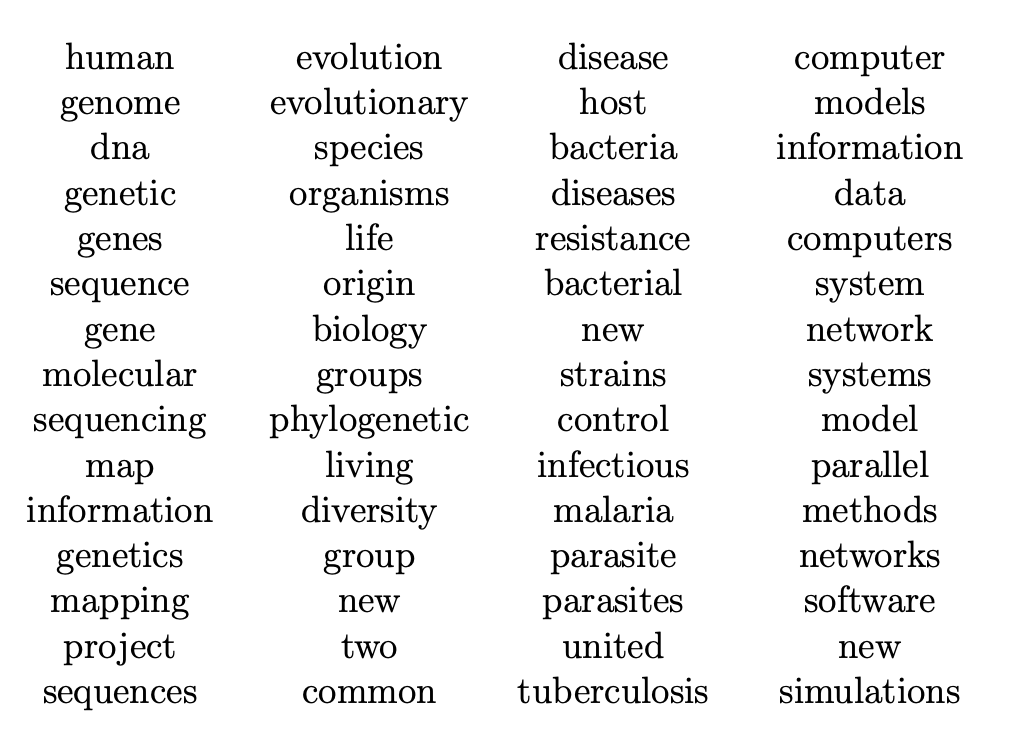
\includegraphics[scale=0.45]{topic_eg}
	
	\end{figure}
}

\frame{ \frametitle{Probabilistic Topic Models}
\begin{figure}
	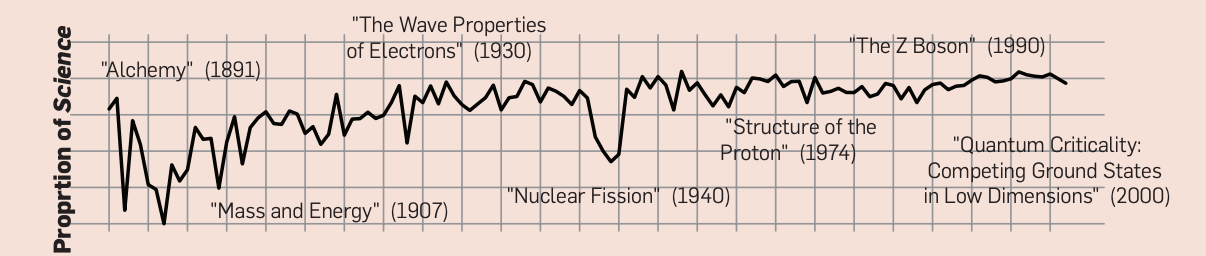
\includegraphics[scale=0.45]{time_eg2}
	
	\end{figure}
}

\frame{ \frametitle{Probabilistic Topic Models}
\begin{figure}
	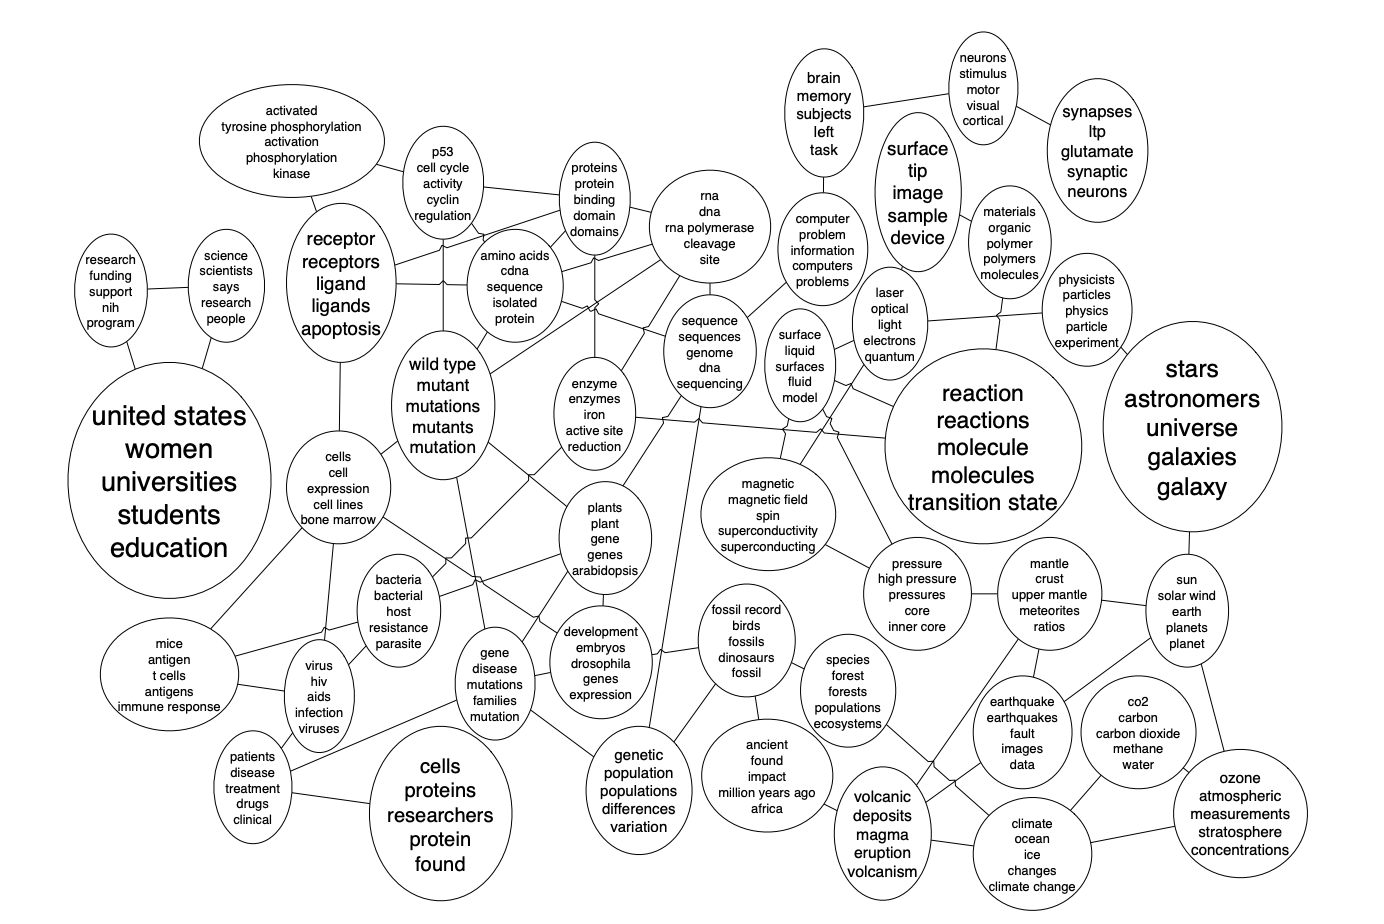
\includegraphics[scale=0.45]{corr_eg}
	
	\end{figure}
}

\frame{ \frametitle{Probabilistic Models}
\begin{figure}
	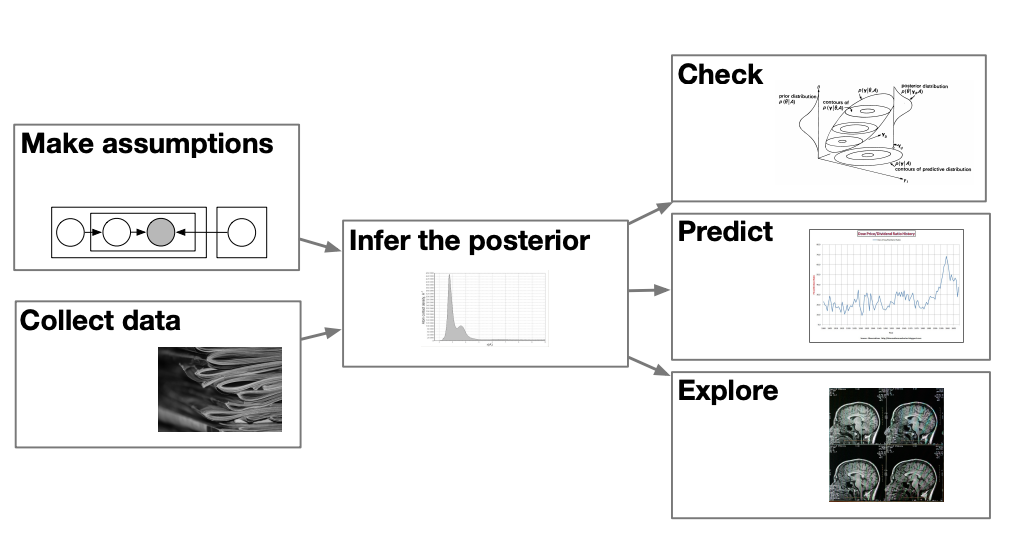
\includegraphics[scale=0.45]{prob_model}
	
	\end{figure}
}



\frame[<+->]{ \frametitle{Latent Dirichlet allocation (LDA)}
\begin{itemize}
\item Motivation  is that documents show multiple topics. 

\item For example, in “Seeking Life’s Bare (Genetic) Necessities,” is about using data analysis to determine the number of genes an organism needs to survive (in an evolutionary sense).
\item Highlighted words related to  data analysis:
\textbf{computer} and \textbf{prediction}, are highlighted in blue;  \\
and evolutionary biology: \textbf{life} and \textbf{organism}, in pink; 
\item LDA is described by its generative process, the imaginary random process by which the model
assumes the documents arose.
\item We denote a topic to be a distribution over a fixed vocabulary. 
\item For example, the genetics topic contains words about genetics with high probability.
\item  We assume that these topics are specified before any data has been generated.
\end{itemize}

}

\frame[<+->]{ \frametitle{LDA}
\begin{figure}
	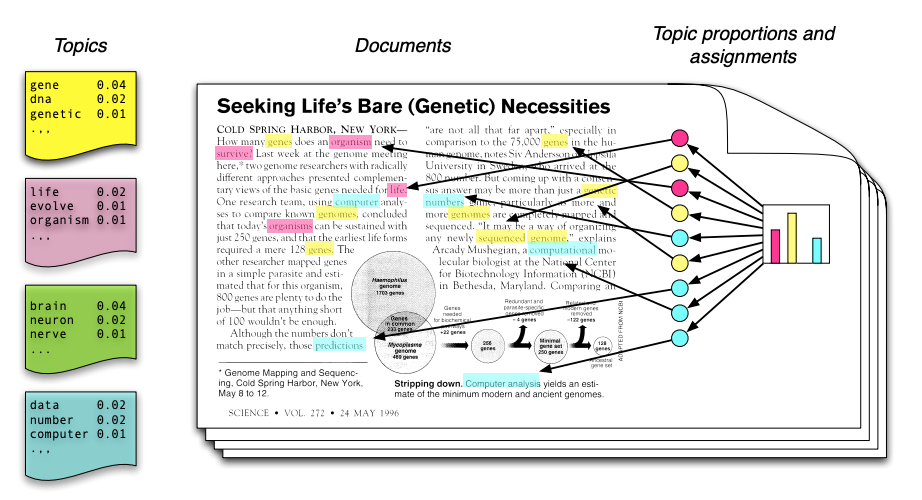
\includegraphics[scale=0.60]{lda}
	
	\end{figure}
\footnotesize{
\begin{itemize}
\item Each topic is a distribution over words
\item Each document is a mixture of corpus-wide topics
\item Each word is drawn from one of those topics
\end{itemize}
}
}

\frame[<+->]{ \frametitle{LDA Objective}
\begin{figure}
	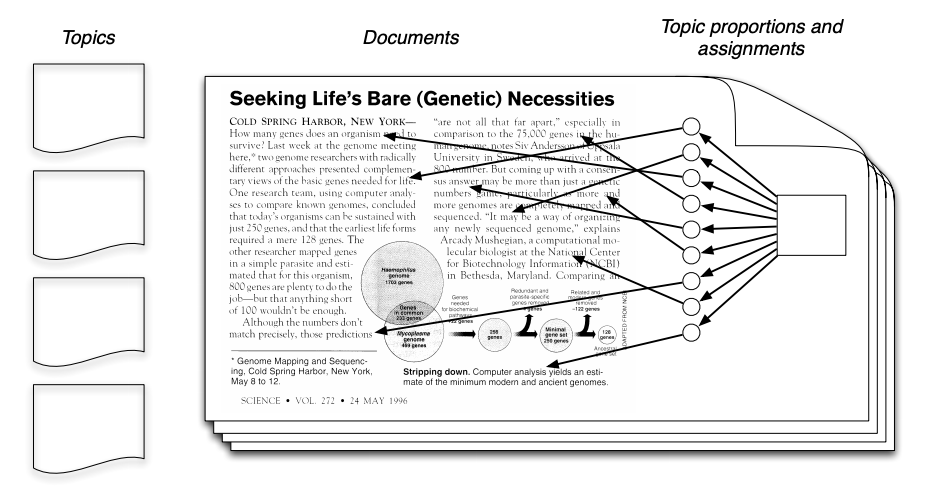
\includegraphics[scale=0.5]{lda_post}
	
	\end{figure}
\begin{itemize}
\item We only observe the documents
\item The conditional distribution of the topic structure given the observed documents
\end{itemize}
}

\frame[<+->]{ \frametitle{LDA}
For each document :
\begin{enumerate}
\item Randomly choose a distribution over topics. 
\item For each word in the document:
\begin{itemize}
\item[a] Randomly choose a topic from the distribution over topics in
step 1.
\item[b] Randomly choose a word from the corresponding distribution over the vocabulary
\end{itemize}
\end{enumerate}
\begin{itemize}
\item Each document exhibits the topics in different proportion (step1); each word in each document is drawn from one of the topics (step 2b), where the selected topic is chosen from the per-document distribution over topics (step 2a)
\item From the example article, the distribution over topics would place probability on genetics, data analysis, and evolutionary biology, and each word
is drawn from one of those three topics.
\end{itemize}


}


\frame[<+->]{ \frametitle{LDA PGM}
\begin{figure}
	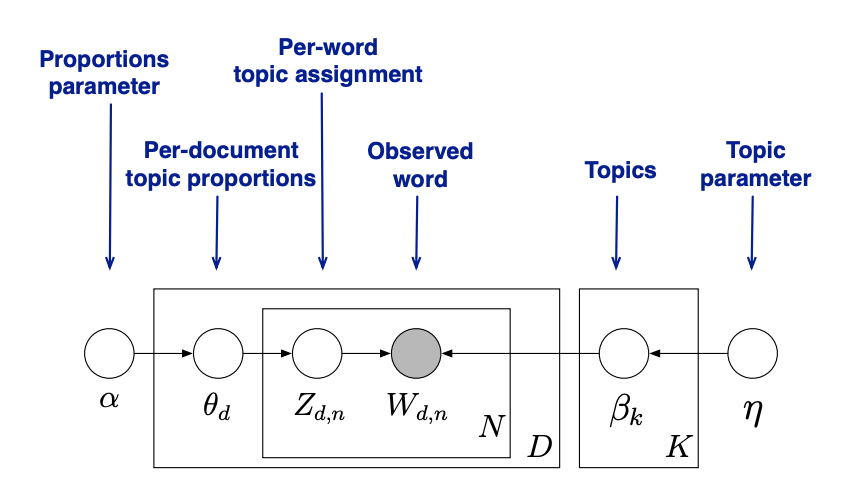
\includegraphics[scale=0.5]{lda_var}
	
	\end{figure}
\begin{itemize}
\item 
\end{itemize}
}


\frame[<+->]{ \frametitle{LDA PGM}
\begin{figure}
	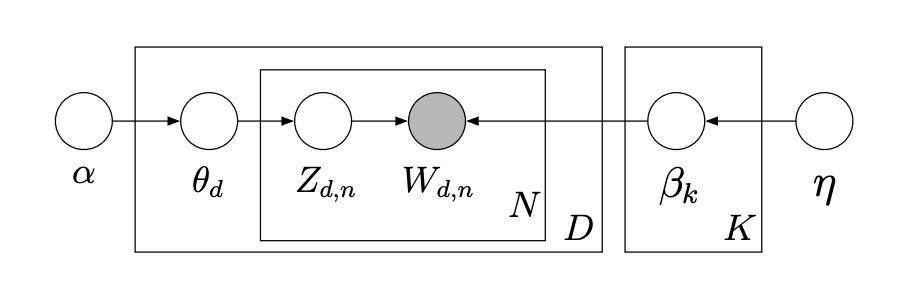
\includegraphics[scale=0.5]{lda_pgm}
	
	\end{figure}
\begin{itemize}
\item This joint defines a posterior, $p(\theta ,z, \beta |w)$.
\item From a collection of documents, infer
\item Per-word topic assignment $z_{d,n}$
\item Per-document topic proportions $\theta_d$
\item Per-corpus topic distributions $\beta_k$
\item Then use posterior expectations to perform the task at hand: information retrieval, document similarity, exploration, and others.
\end{itemize}
}


\frame{ \frametitle{Dirichlet distribution}
\begin{itemize}
\item The Dirichlet distribution is an exponential family distribution over the
simplex, i.e., positive vectors that sum to one \\
\begin{equation}
p(\theta | \alpha)=\frac{\Gamma\left(\sum_{i} \alpha_{i}\right)}{\prod_{i} \Gamma\left(\alpha_{i}\right)} \prod_{i} \theta_{i}^{\alpha_{i}-1}
\end{equation}
\item  It is conjugate to the multinomial. Given a multinomial observation, the
posterior distribution of $\theta$ is a Dirichlet.
\item The parameter $\alpha$ controls the mean shape and sparsity of $\theta$ .
\item  The topic proportions are a K dimensional Dirichlet. The topics are a V dimensional Dirichlet.
\item  The alpha controls the mixture of topics for any given document. 
\end{itemize}
}

\frame{ \frametitle{Dirichlet distribution}
\scalebox{0.65}{
\animategraphics[loop,controls,width=\linewidth]{10}{dirichlet/dir-}{0}{15}
}

}

\frame[<+->]{ \frametitle{Dirichlet distribution}
\begin{itemize}
\item At low alpha values (less than one), most of the topic distribution samples are in the corners (near the topics).


\item At alpha equal to one, any space on the surface of the triangle (3-simplex) is fair game (uniformly distributed). You could equally likely end up with a sample favoring only one topic, a sample that gives an even mixture of all the topics, or something in between.

\item For alpha values greater than one, the samples start to congregate to the center. This means that as alpha gets bigger, your samples will more likely be uniform or an even mixture of all the topics.

\end{itemize}
}



\frame{ \frametitle{Working}
LDA trades off two goals.
\begin{itemize}
\item \textbf{(1)} For each document, allocate its words to as few topics as possible.\\
\textbf{(2)} For each topic, assign high probability to as few terms as possible.

\item Putting a document in a single topic makes 2 hard:
All of its words must have probability under that topic.
\item Putting very few words in each topic makes 1 hard:
To cover a document's words, it must assign many topics to it.
\item Trading off these goals finds groups of tightly co-occurring words.
\end{itemize}
}

\frame{ \frametitle{Posterior Inference}
\begin{figure}
	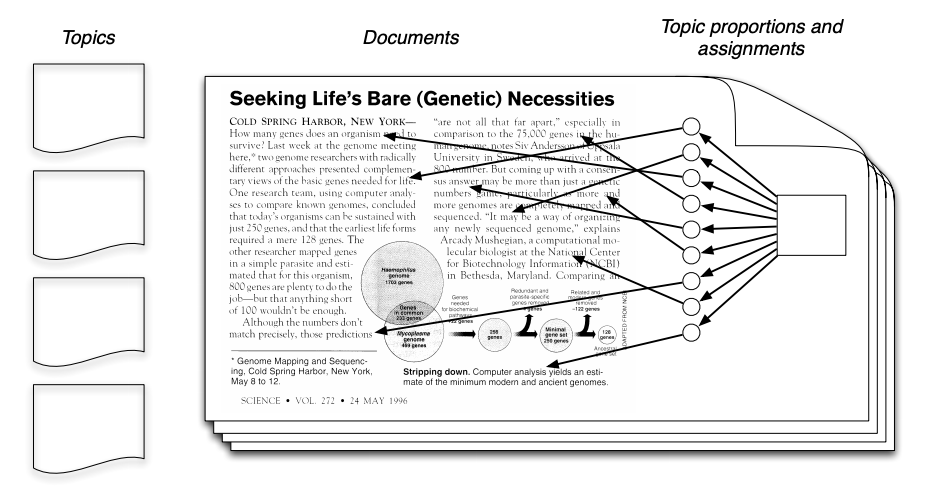
\includegraphics[scale=0.5]{lda_post}
	
	\end{figure}
\begin{itemize}
\item Our goal is to compute the distribution of the hidden variables conditioned on the documents \\
p(topics, proportions, assignments|documents)
\end{itemize}
}



\frame{ \frametitle{Posterior Inference}
\begin{figure}
	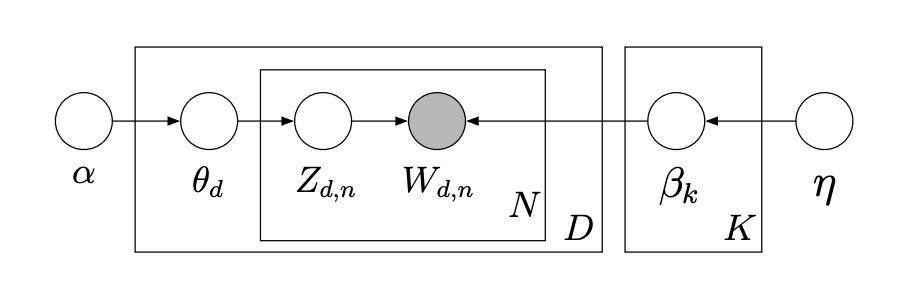
\includegraphics[scale=0.5]{lda_pgm}
	
	\end{figure}
\begin{itemize}

\item The joint distribution of the latent variables and documents is \\
$\prod_{i=1}^{K} p\left(\beta_{i} | \eta\right) \prod_{d=1}^{D} p\left(\theta_{d} | \alpha\right)\left(\prod_{n=1}^{N} p\left(z_{d, n} | \theta_{d}\right) p\left(w_{\alpha, n} | \beta_{1 : k, z_{d, n}}\right)\right)$
\item The posterior of the latent variables given the documents is \\
$p(\beta, \theta, \mathbf{z} | \mathbf{w})$
\end{itemize}
}

\frame{ \frametitle{Posterior Inference}

\begin{itemize}
\item 
$p(\beta, \theta, \mathbf{z} | \mathbf{w}) = \frac{p(\beta, \theta, \mathbf{z}, \mathbf{w})}{\int_{\beta} \int_{\theta} \sum_{\mathbf{z}} p(\beta, \theta, \mathbf{z}, \mathbf{w})}$
\item The denominator, the marginal $p(w)$ is intractable
\end{itemize}
}

\frame{ \frametitle{Posterior Inference}
\begin{figure}
	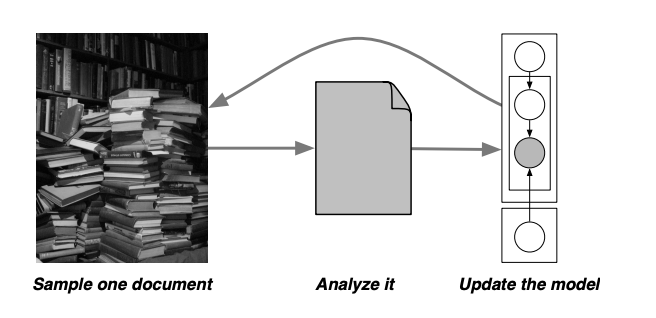
\includegraphics[scale=0.5]{vi_lda}
	
	\end{figure}
\begin{itemize}
\item Condition on large data sets and approximate the posterior.
\item Variational inference, we optimize over a family of distributions to find the member closest in KL divergence to the posterior.
\end{itemize}
}


\frame{ \frametitle{Posterior Inference}
\begin{figure}
	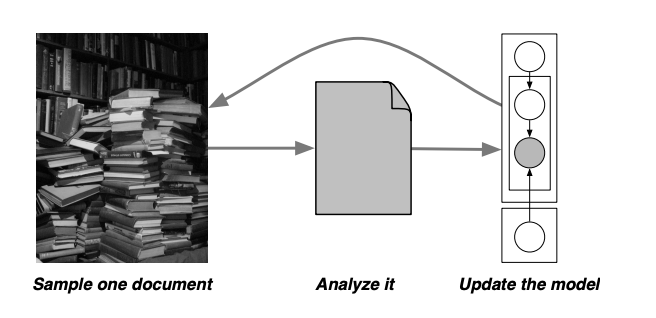
\includegraphics[scale=0.5]{vi_lda}
	
	\end{figure}
\begin{enumerate}
\item Sample a document $w_d$ from the collection
\item Infer how $w_d$ exhibits the current topics
\item Create intermediate topics, formed as though the $w_d$ is the only document.
\item Adjust the current topics according to the intermediate topics.
\item Repeat.
\end{enumerate}

}

\frame{ \frametitle{Mean-field variational inference for LDA}
\begin{figure}
	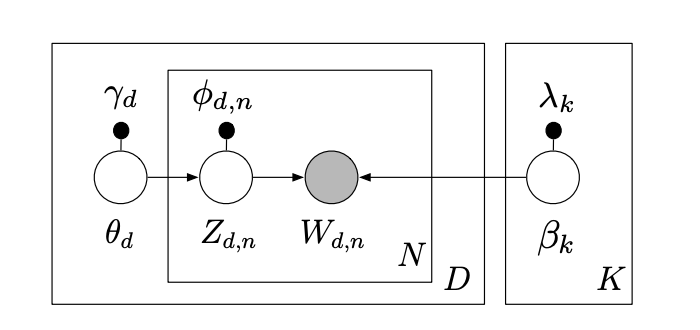
\includegraphics[scale=0.5]{vi2-lda}
	
	\end{figure}
\begin{enumerate}
\item Document variables: Topic proportions $\theta$ and topic assignments $z_{1:N}$ .
\item Corpus variables: Topics $\beta_{1:K}$
\item The variational approximation  is: \\
$q(\boldsymbol{\beta}, \boldsymbol{\theta}, z)=\prod_{k=1}^{K} q\left(\beta_{k} | \lambda_{k}\right) \prod_{d=1}^{D} q\left(\theta_{d} | \gamma_{d}\right) \prod_{n=1}^{N} q\left(z_{d, n} | \phi_{d, n}\right)$
\end{enumerate}

}


\frame{ \frametitle{Mean-field variational inference for LDA}
\begin{figure}
	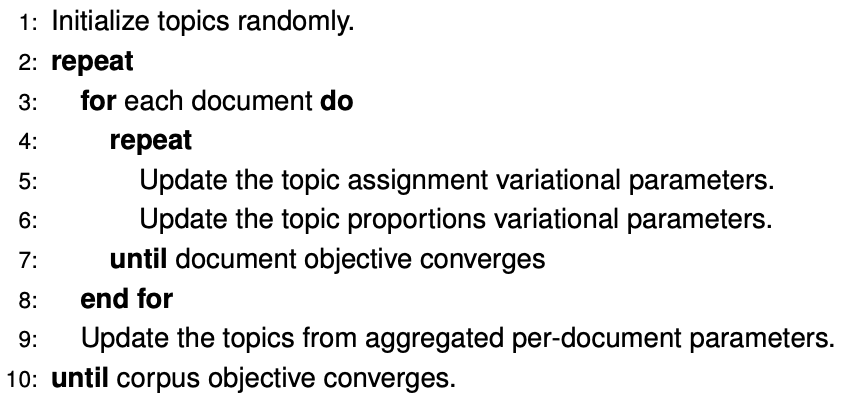
\includegraphics[scale=0.55]{algovi_lda}
	
	\end{figure}


}






\frame{ \frametitle{LDA Extensions}
\begin{figure}
	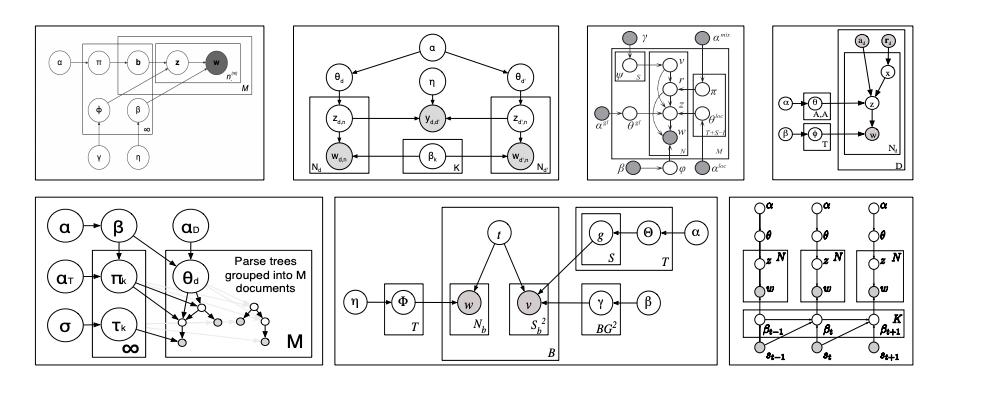
\includegraphics[scale=0.65]{lda_ext}
	
	\end{figure}
}



\frame[<+->]{ \frametitle{Correlated topic models}
\begin{figure}
	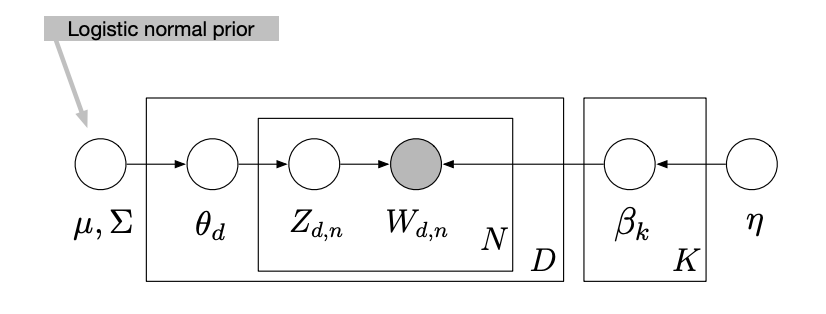
\includegraphics[scale=0.45]{corr_lda}
	
	\end{figure}
\begin{itemize}
\item Draw topic proportions from a logistic normal
\item Allows topic occurrences to have correlation.
\item Gives a map of topics and how they are related
\item Better fit for observed data, but computation is more complex
\end{itemize}
}

\frame[<+->]{ \frametitle{Dynamic topic models}

\begin{itemize}
\item LDA assumes that the order of documents does not matter.
\item Corpora span hundreds of years
\end{itemize}
\begin{figure}
	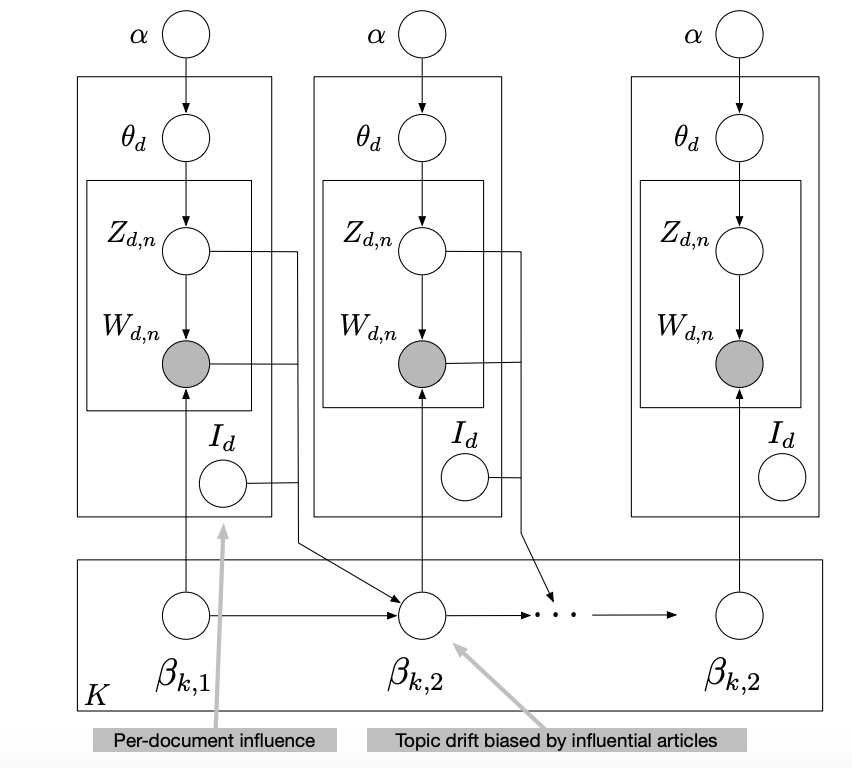
\includegraphics[scale=0.40]{dyn_lda1}
	
	\end{figure}

}

\frame[<+->]{\frametitle{Dynamic topic models}
\begin{itemize}
\item Each document has an influence score $Id$.
\item  Each topic  is biased with the documents with high influence.
\item The posterior of the influence scores could find articles that best explain the changes in language.
\end{itemize}

}

\frame{ \frametitle{Dynamic topic models}
\begin{figure}
	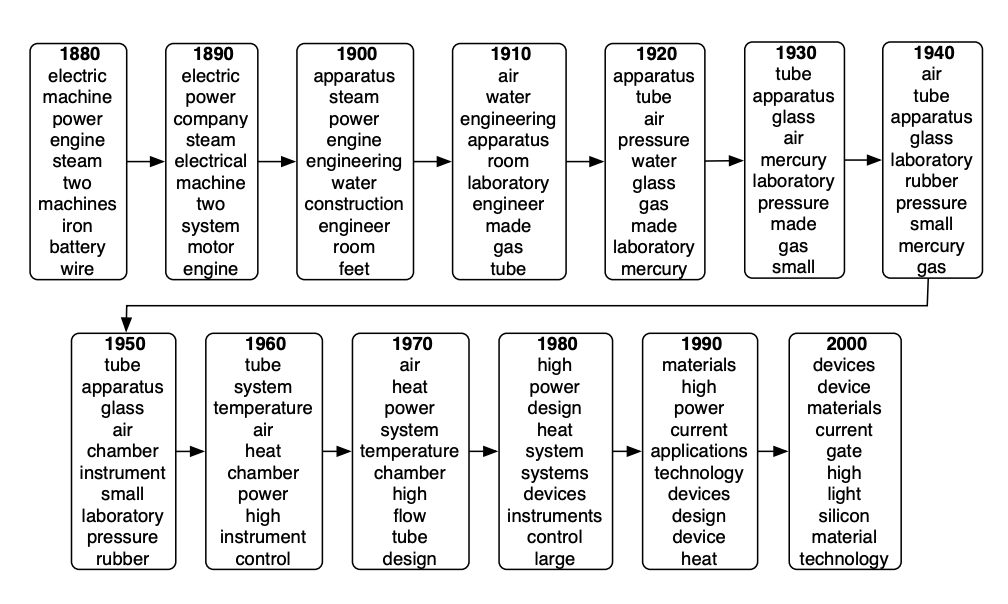
\includegraphics[scale=0.55]{dyn_lda2}
	
	\end{figure}
}





\section{Neural Variational Inference for Text Processing}


\frame[<+->]{ \frametitle{Neural Variational Inference for Text Processing}

\begin{itemize}

\item Neural variational framework for generative models of documents  based on the variational auto-encoder.
\item NVDM is a generative model of text which aims to extract a continuous semantic latent
variable for each document.
\item Model is denoted by variational auto-encoder: 
\item MLP encoder (inference)  compresses the bag-of-words document representation into a continuous latent distribution,
\item  Softmax decoder (generative model) reconstructs the document by generating the words independently.

\end{itemize}
\ack{\citep{pmlr-v48-miao16}}
}


\frame[<+->]{ \frametitle{Neural Variational Inference for Text Processing}

\begin{figure}
	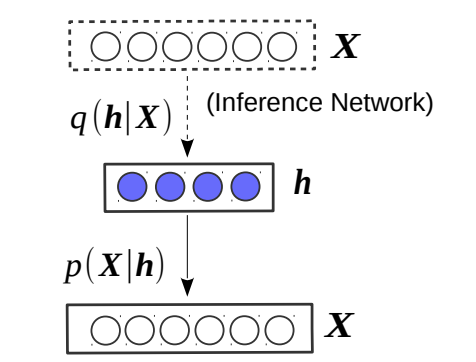
\includegraphics[scale=0.65]{nvdm}
	
	\end{figure}

}

\frame[<+->]{ \frametitle{Neural Variational Inference for Text Processing}

\begin{itemize}

\item Let $X in R^{|V |}$ be the bag-of-words representation of a document and $x_i in R^{|V |}$ be the one-hot
representation of the word at position $i$.
\item MLP encoder $q(z|x)$ compresses document representations into continuous hidden vectors 
\item  Softmax decoder $p(\boldsymbol{x} | \boldsymbol{z})=\prod_{i=1}^{N} p\left(\boldsymbol{x}_{i} | \boldsymbol{z}\right)$ reconstructs the documents by
independently generating the words. 
\item We derive the lower bound: \\
$\mathcal{L}=\mathbb{E}_{q_{\phi}(\boldsymbol{z} | \boldsymbol{x})}\left[\sum_{i=1}^{N} \log p_{\theta}\left(\boldsymbol{x}_{i} | \boldsymbol{z}\right)\right]-D_{\mathrm{KL}}(q_{\phi}(\boldsymbol{z} | \boldsymbol{x}) \| p(\boldsymbol{z}))$ \\
where N is the number of words in the document 
\end{itemize}

}



\frame[<+->]{ \frametitle{Data}

\begin{itemize}

\item Standard news corpora: 

\item  20NewsGroups is a collection of newsgroup documents, consisting of 11,314 training and 7,531 test articles.
\item   Reuters RCV1-v2 is a large collection from Reuters newswire stories with 794,414 training and 10,000 test cases.
\item  The vocabulary size of these two datasets are set as 2,000 and 10,000
\end{itemize}

}

\frame[<+->]{ \frametitle{Results}

\begin{figure}
	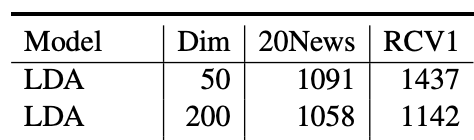
\includegraphics[scale=0.65]{results1_nvdm} \\
	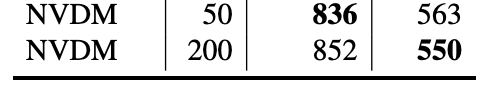
\includegraphics[scale=0.65]{results2_nvdm} 
	
	\end{figure}
\begin{itemize}

\item perplexity is computed $ppl= \exp \left(-\frac{1}{D} \sum_{n}^{N_{d}} \frac{1}{N_{d}} \log p\left(\boldsymbol{x}_{d}\right)\right)$, where D is the number
of documents, $N_d$ represents the length of the dth document.
\item Since $log p(x)$   in the NVDM is the variational lower bound (which is an upper bound on perplexity). 
\end{itemize}

}


\frame[<+->]{ \frametitle{Results}
The topics learned by NVDM on 20News
\begin{figure}
	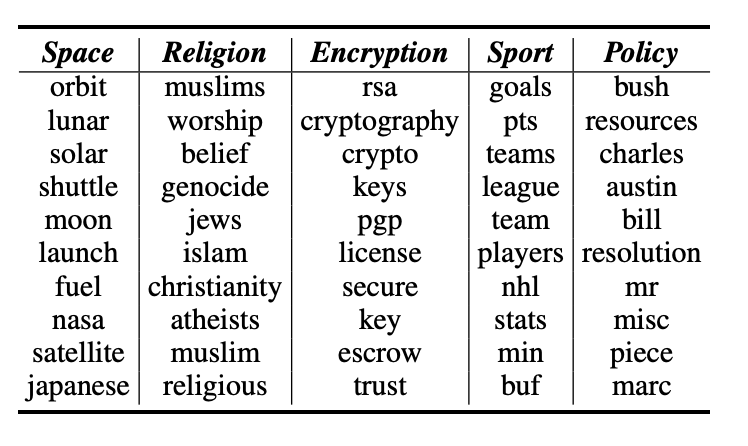
\includegraphics[scale=0.65]{results3_nvdm} 
	
	\end{figure}
}

\section{Discovering Discrete Latent Topics}

\frame[<+->]{ \frametitle{Discovering Discrete Latent Topics }

\small{
\begin{itemize}

\item  Introduce a neural network to parameterise the multinomial topic distribution
\begin{equation}
\begin{aligned} \theta_{d} \sim \mathrm{G}\left(\mu_{0}, \sigma_{0}^{2}\right), & \text { for } d \in D \\ z_{n} \sim \operatorname{Multi}\left(\theta_{d}\right), & \text { for } n \in\left[1, N_{d}\right] \\ w_{n} \sim \operatorname{Multi}\left(\beta_{z_{n}}\right), & \text { for } n \in\left[1, N_{d}\right] \end{aligned}
\end{equation}
\item $G(\mu_0, \sigma_0^2)$ is composed of a NN $\theta = g(x)$ conditioned on a isotropic Gaussian $x \sim \mathcal N (\mu_0, \sigma_0^20)$
\item Gaussian Softmax Construction  pass a Gaussian random vector through a softmax function to parameterise the multinomial document topic distributions. \\
\begin{equation}
\begin{array}{c}{x \sim \mathcal{N}\left(\mu_{0}, \sigma_{0}^{2}\right)} \\ {\theta=\operatorname{softmax}\left(W_{1}^{T} x\right)}\end{array}
\end{equation}

\end{itemize}
}

}


\frame[<+->]{ \frametitle{Discovering Discrete Latent Topics}

\begin{figure}
	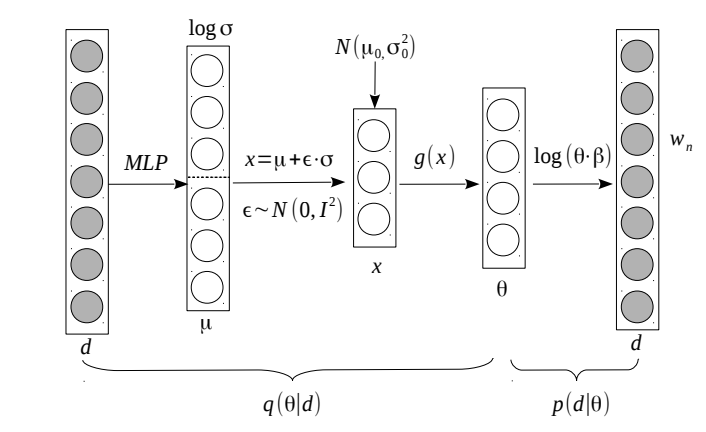
\includegraphics[scale=0.65]{miao1} 
	
	\end{figure}
\ack{\citep{DBLP:journals/corr/MiaoGB17}}
}

\frame[<+->]{ \frametitle{Discovering Discrete Latent Topics}

\begin{itemize}

\item Neural Topic Models with a finite number of topics K.
\item  The topic distribution over words given a topic assignment $z_n$ is\\
$p(w_n | \beta, z_n) = \operatorname{Multi}(\beta_{z_n} ) $. 
\item Introduce topic vectors $t \in R^{K \times H}$
\item  word vectors $v \in R^{V \times H}$ 
\item and generate the topic distributions over words by:\\
$\beta_{k}=\operatorname{softmax}\left(v \cdot t_{k}^{T}\right)$ \\
$\beta \in R^{K \times V}$ is the  semantic similarity between topics and words. 

\end{itemize}

}

\frame[<+->]{ \frametitle{Discovering Discrete Latent Topics}

\begin{itemize}

\item With lower bound: \\
$\mathcal{L}_{d} =\sum_{n=1}^{N}\left[\log p\left(w_{n} | \beta, \hat{\theta}\right)\right]-D_{K L}[q(x | d) \| p(x)]$
\item 
\begin{equation}
\begin{aligned} \log p\left(w_{n} | \beta, \hat{\theta}\right) &=\log \sum_{z_{n}}\left[p\left(w_{n} | \beta_{z_{n}}\right) p\left(z_{n} | \hat{\theta}\right)\right] \\ &=\log (\hat{\theta} \cdot \beta) \end{aligned}
\end{equation}
\item[CON]  addition of topic diversity regularisation to the objective
\end{itemize}

}

\frame[<+->]{ \frametitle{Discovering Discrete Latent Topics}

\begin{itemize}

\item Unbounded neural topic models the topics $t \in  R^{\infty \times H}$ are dynamically generated by
$\text{RNN}_{\text{Topic}}$ The generation of $\beta$  is as follows:
\begin{equation}
\begin{aligned} t_{k} &=\operatorname{RNN}_{\text { Topic }}\left(t_{k-1}\right) \\ \beta_{k} &=\operatorname{softmax}\left(v \cdot t_{k}^{T}\right) \end{aligned}
\end{equation}
\item where  $v$ represents the word vectors, $t_k$ is the kth topic generated by RNN
\item  If $I > \gamma$, we increase the active number of topics $i$ by 1,\\
$\mathcal{I}=\sum_{d}^{D}\left[\mathcal{L}_{d}^{i}-\mathcal{L}_{d}^{i-1}\right] / \sum_{d}^{D}\left[\mathcal{L}_{d}^{i}\right]$
\end{itemize}
}


\frame[<+->]{ \frametitle{Discovering Discrete Latent Topics}


\begin{figure}
	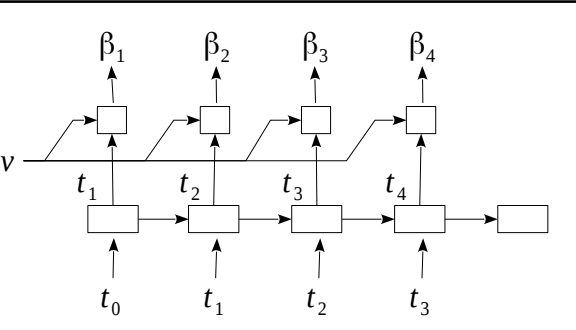
\includegraphics[scale=0.65]{unb} 
	
	\end{figure}
\begin{itemize}

\item 
\begin{equation}
\begin{aligned} t_{k} &=\operatorname{RNN}_{\text { Topic }}\left(t_{k-1}\right) \\ \beta_{k} &=\operatorname{softmax}\left(v \cdot t_{k}^{T}\right) \end{aligned}
\end{equation}
\end{itemize}
}



\frame[<+->]{ \frametitle{Results}
\begin{figure}
	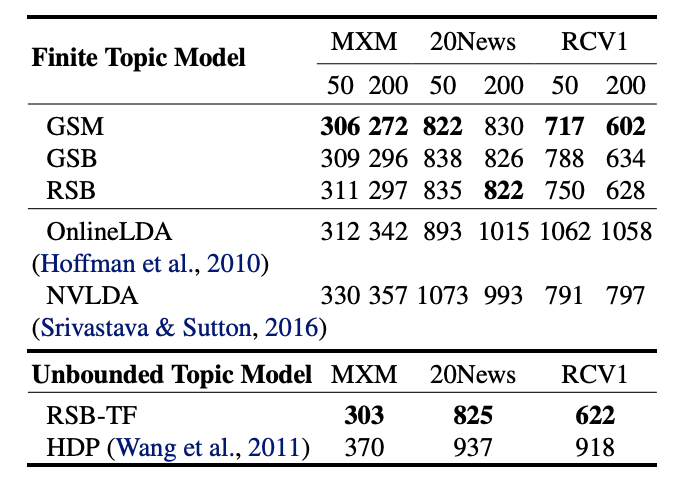
\includegraphics[scale=0.65]{results_unb} 
	
	\end{figure}
\begin{itemize}

\item *MXM the Million Song Dataset with 210,519 training and 27,143 testing
\end{itemize}

}

\frame[<+->]{ \frametitle{Results}
\begin{figure}
	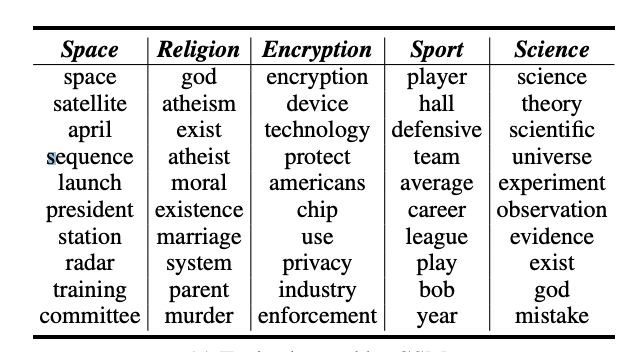
\includegraphics[scale=0.8]{topics_unb} 
	
	\end{figure}


}

\section{LDA VAE}

\frame[<+->]{ \frametitle{LDA VAE}

\begin{itemize}
\item Effective VAE based model for LDA
\item Dirichlet within VAE is difficult to develop an effective reparameterisation function \\
Solve by constructing a Laplace approximation to the Dirichlet prior.
\item This approximation to the Dirichlet  results in the distribution over the softmax variables

\end{itemize}


\ack{\citep{Srivastava2017AutoencodingVI}}
}

\frame[<+->]{ \frametitle{Laplace approximation}
\begin{itemize}
\item Approximation in  the softmax basis instead of the simplex.
\item  Dirichlet probability density function over the softmax variable $h$ is:
\begin{equation}
P(\theta(\mathbf{h}) | \alpha)=\frac{\Gamma\left(\sum_{k} \alpha_{k}\right)}{\prod_{k} \Gamma\left(\alpha_{k}\right)} \prod_{k} \theta_{k}^{\alpha_{k}} g\left(\mathbf{1}^{T} \mathbf{h}\right)
\end{equation}
\item Here $\theta = \sigma(h)$, where $\sigma(\cdot)$ represents the softmax function
\end{itemize}


}


\frame[<+->]{ \frametitle{LDA VAE}

\begin{itemize}

\item Approximation to the Dirichlet  results in the distribution over the softmax variables
h as a multivariate normal with mean $\mu_1$ and covariance matrix $\Sigma_1$ where:
\begin{equation}
\begin{aligned} \mu_{1 k} &=\log \alpha_{k}-\frac{1}{K} \sum_{i} \log \alpha_{i} \\ \Sigma_{1 k k} &=\frac{1}{\alpha_{k}}\left(1-\frac{2}{K}\right)+\frac{1}{K^{2}} \sum_{i} \frac{1}{\alpha_{k}} \end{aligned}
\end{equation}
\end{itemize}

}


\frame[<+->]{ \frametitle{LDA VAE}
\footnotesize{
\begin{itemize}
\item Approximate of $p(\theta | \alpha)$ with $\hat{p}\left(\theta | \mu_{1}, \Sigma_{1}\right)=\mathcal{L} \mathcal{N}\left(\theta | \mu_{1}, \Sigma_{1}\right)$
\item where LN is a logistic normal distribution with parameters  $\mu_1$, $\Sigma_1$ for k (number of topics).
\item and ELBO:
\begin{equation}
\begin{array}{r}{L(\boldsymbol{\Theta})=\sum_{d=1}^{D}\left[-\left(\frac{1}{2}\left\{\operatorname{tr}\left(\boldsymbol{\Sigma}_{1}^{-1} \boldsymbol{\Sigma}_{0}\right)+\left(\boldsymbol{\mu}_{1}-\boldsymbol{\mu}_{0}\right)^{T} \boldsymbol{\Sigma}_{1}^{-1}\left(\boldsymbol{\mu}_{1}-\boldsymbol{\mu}_{0}\right)-K+\log \frac{\left|\boldsymbol{\Sigma}_{1}\right|}{\left|\boldsymbol{\Sigma}_{0}\right|}\right\}\right)\right.} \\ {+\mathbb{E}_{\boldsymbol{\epsilon} \sim \mathcal{N}(0, I)}\left[\mathbf{w}_{d}^{\top} \log \left(\sigma(\boldsymbol{\beta}) \sigma\left(\boldsymbol{\mu}_{0}+\boldsymbol{\Sigma}_{0}^{1 / 2} \boldsymbol{\epsilon}\right)\right)\right] ]}\end{array}
\end{equation}
\item with $\mu_{0}=f_{\mu}(\mathbf{w}, \boldsymbol{\delta})$ and $\boldsymbol{\Sigma}_{0}=\operatorname{diag}\left(f_{\Sigma}(\mathbf{w}, \boldsymbol{\delta})\right)$
\end{itemize}
}
}


\frame[<+->]{ \frametitle{Architecture}

\begin{figure}
	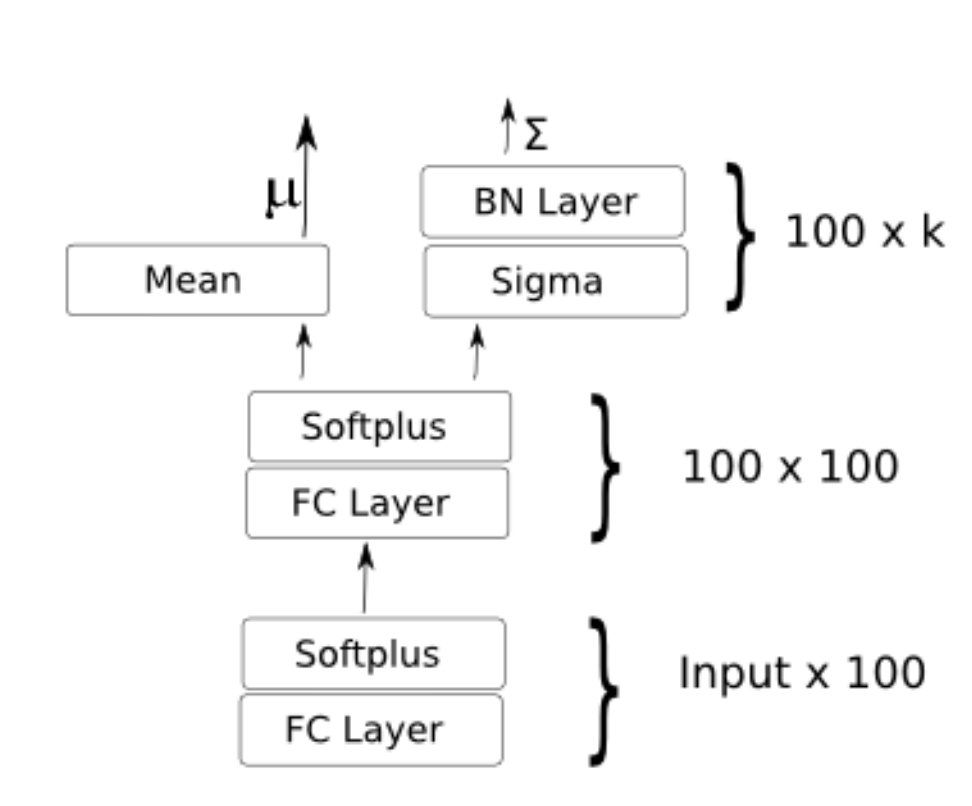
\includegraphics[scale=0.45]{ldavae_arch} 
	
	\end{figure}

}

\frame[<+->]{ \frametitle{Results}

\begin{figure}
	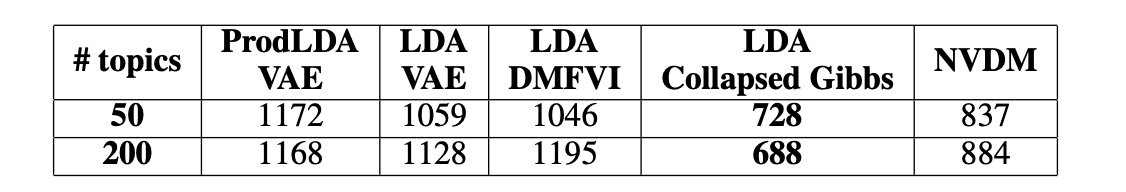
\includegraphics[scale=0.6]{results_ldavae} 
	
	\end{figure}
ppl 20 Newsgroups
}



\frame[<+->]{ \frametitle{Results}

\begin{figure}
	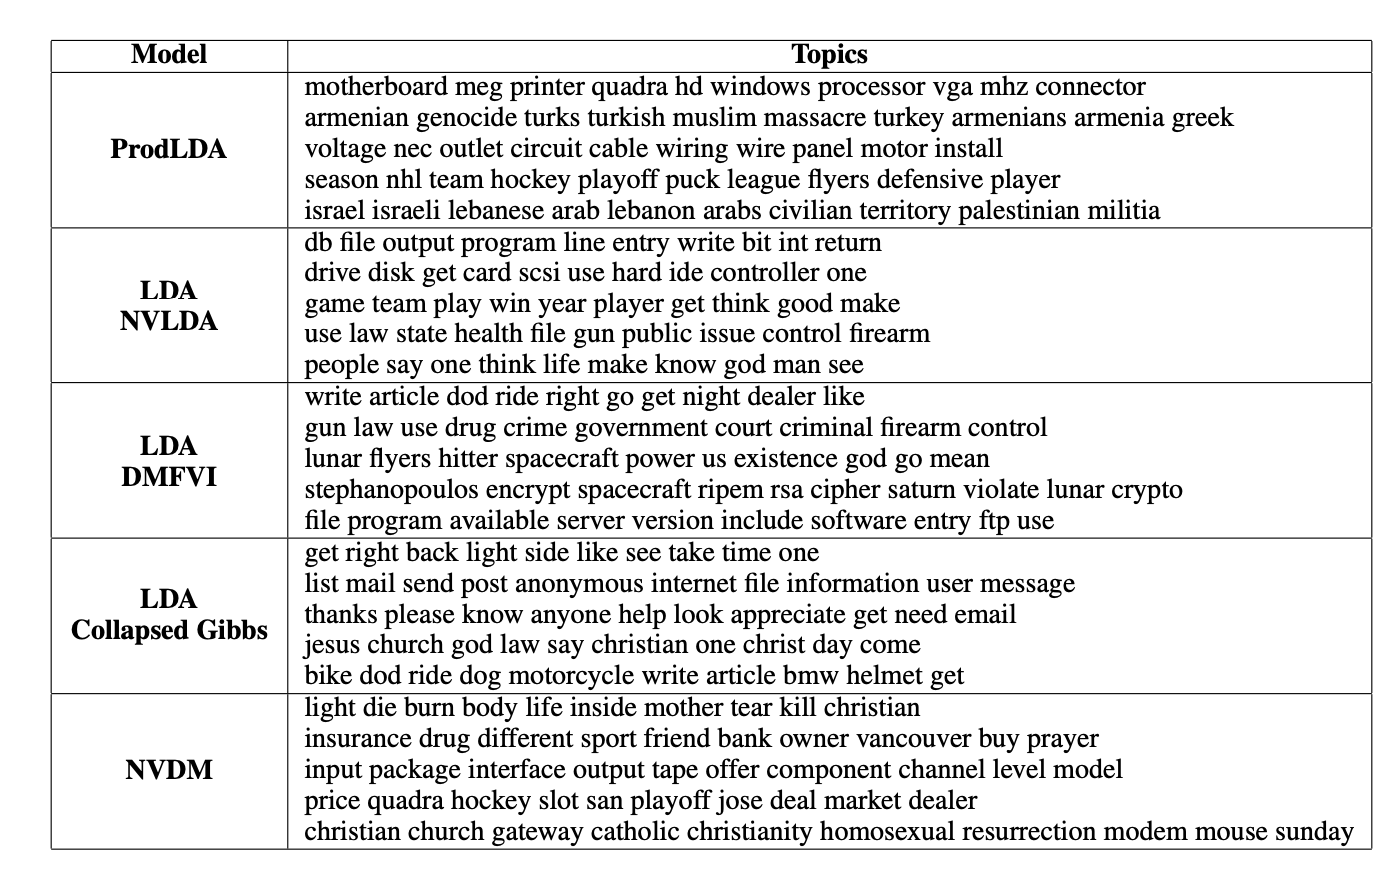
\includegraphics[scale=0.40]{ldavae_topics} 
	
	\end{figure}

}


\section*{References}
	
	%\input{backup}


	\frame[allowframebreaks]{ \frametitle{References}
	
        \bibliographystyle{plainnat}
        \bibliography{BIB}
	}


\end{document}
\grid
